The PC environment had morphed significantly between the development of Wolfenstein 3D in 1991 and the development of Doom in 1993. However a machine could still be summarize by seven subsystems \circled{1}~Inputs, \circled{2}~CPU, \circled{3}~RAM, \circled{4}~Bus, \circled{5}~Video~output, \circled{6}~Audio~output and \circled{7}~Operating~System.\\
\par
\pngdrawing{pc_components}{The six components of an IBM PC.}
\par
Before describing each components in details, it is important to remind the reader that despite its improvements, the IBM PC of 1993 was not something built for 3D video games. These were machine originally designed to do word processing, spreadsheet and sometimes display a nice static image or graph. The builders never had in mind something refreshing the screen at 70Hz.\\
\par Each elements in the machine attested of the original intend, with a CPU very good at doing the wrong thing, a VGA with no double buffering capabilities and a primitive sound emitter only capable of one pitch. Any sane programmer would have ran away from a machine so ill-fated. This is what the few courageous developers of the time had to deal with.\\
\par
With this reminder out of the way, let's discover the state of the art of a PC from 1993 by looking at the component connecting everything together. The best seller motherboard of 1993, the PX486P3 by QDI Computer, Inc\footnote{Again, a canadian company :) !}.\\
\par

\cfullimage{PX486P3/b-486-px486p3}{Motherboard PX486P3 by QDI Computer, Inc}
\par
The most prominent novelty is of course the Intel i486 CPU. However by looking closer we can notice three less visible feature which would prove of paramount importance for the design of \doom. If the black extension connectors show the traditional ISA bus ports, a 8 bit one (\circled{1}), two dual slot 16 bit (\circled{2}) we can also see a new type of connector with three slots (\circled{3}). These are VBL\footnote{Video Local Bus.}, a new type of bus up to 20x faster than ISA. Next in the upper right we can see large rows of black chips, a new type of RAM called sRAM\footnote{Static RAM}, up to 10x faster than dRAM\footnote{Dynamic RAM} aiming at avoiding CPU stalls\footnote{SRAM was expensive and took a lot of space. Despite their size compared to the DRAM (in white), the eight chips could only stored 256 KiB with 20ns access time.}. \\
\par
\drawing{px486p3}{Components diagram of the PX486P3.}
\begin{enumerate}
\item RAM prices had dropped significantly. The standard 2 MiB was not a whooping 4 MiB. 
\item Bandwidth hungry GUI and had lead motherboard manufacturers to come up with a faster bus called VLB.
\item The sound generator ecosystems was even more fragmented than before with more and more manufacturer producing sound cards.
\item Not visible on the drawing, the operating system shortcomings were being addressed by independent developers via something called "DOS eXtenders".
\item Unsurprisingly the impossible to program VGA was still the standard but manufacturers were now competing to produce the faster DACs and \fixme{"RAMDAC"}?.
\item CACHE
\end{enumerate}
Finally in the upper right, two large dRAM banks, allowing 4 30-pin SIMM sockets for a total of up to 32MiB. Indeed the price of RAM was falling and PCs which used to be i386 with 2MiB now came equipped with 4 MiB.\\
\par

\begin{center}
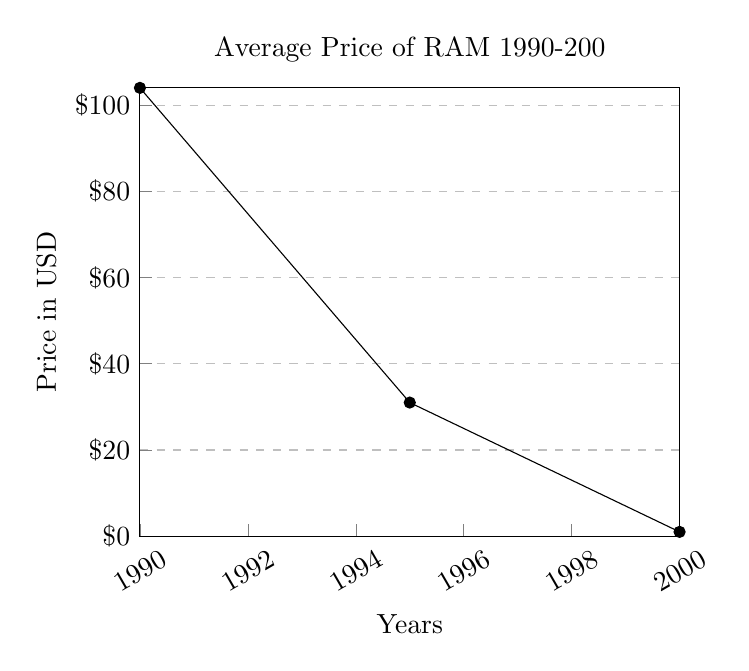
\begin{tikzpicture}

\begin{axis}[
    title={Average Price of RAM 1990-200},
    xlabel={Years},
    xtick pos=left,
    ytick pos=left,
    ylabel={Price in USD},
    yticklabel={${\$\pgfmathprintnumber{\tick}}$},
    xticklabel style={ rotate=30,},
    xticklabel style={/pgf/number format/1000 sep=},
    xmin=1990, xmax=2000,
    ymin=0, ymax=104,
    %xtick={0,20,40,60,80,100},
    %ytick={0,20,40,60,80,100,120},
    legend pos=north west,
    ymajorgrids=true,
    grid style=dashed,
]
 
\addplot[
    color=black,
    mark=*,
    ]
    coordinates {
    (1990,104)(1995,31)(2000,1)
    };
    %\legend{CuSO$_4\cdot$5H$_2$O}
 
\end{axis}
\end{tikzpicture}
\end{center}

Back then, it was a fair assumption to assume the next PC would have twice the processing power and twice the RAM capacity.
\par
\break





